\section{Experimental Results}
\label{sec:experiment}

\setlength{\tabcolsep}{0.5pt}
\begin{figure*}
\begin{center}
\begin{tabular}{ccccccc}
& \multicolumn{3}{c}{\small -------------------- Object 1: dog --------------------} & \multicolumn{3}{c}{\small -------------------- Object 2: cat --------------------} \\
\vspace{-2.5pt}
%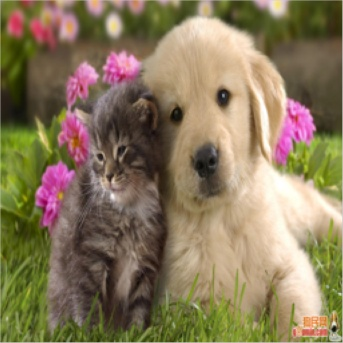
\includegraphics[width=0.14\linewidth,height=0.115\linewidth]{figs/examples/googlenet/oxford/dog-cat1} &
%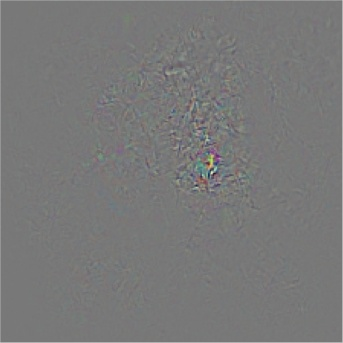
\includegraphics[width=0.14\linewidth,height=0.115\linewidth]{figs/examples/googlenet/oxford/dog-cat1_diff_258} &
%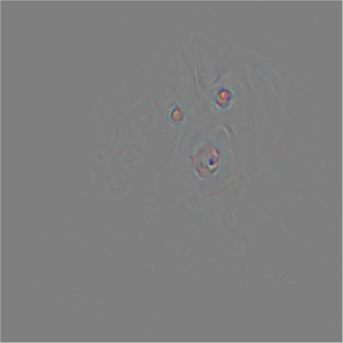
\includegraphics[width=0.14\linewidth,height=0.115\linewidth]{figs/examples/googlenet/deconv/dog-cat1_diff_258} &
%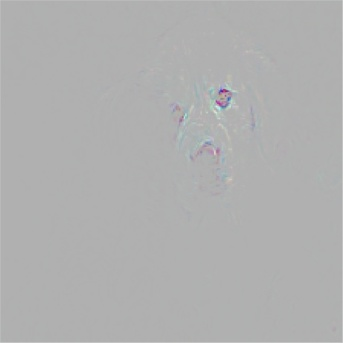
\includegraphics[width=0.14\linewidth,height=0.115\linewidth]{figs/examples/googlenet/soft/dog-cat1_diff_258} &
%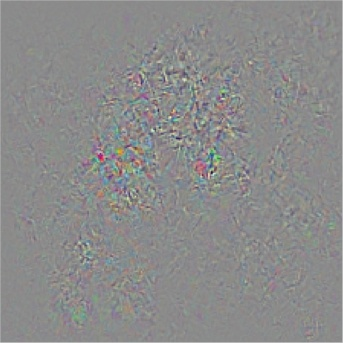
\includegraphics[width=0.14\linewidth,height=0.115\linewidth]{figs/examples/googlenet/oxford/dog-cat1_diff_286} &
%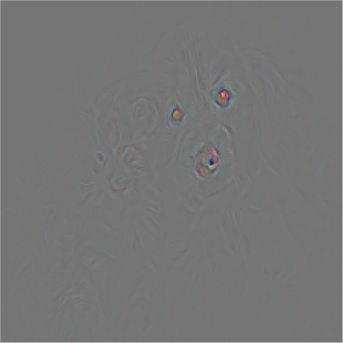
\includegraphics[width=0.14\linewidth,height=0.115\linewidth]{figs/examples/googlenet/deconv/dog-cat1_diff_286} &
%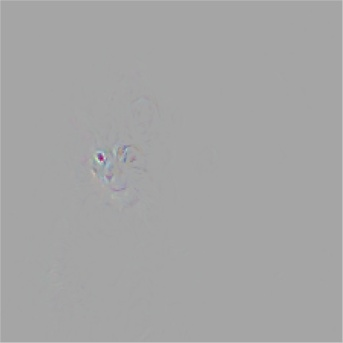
\includegraphics[width=0.14\linewidth,height=0.115\linewidth]{figs/examples/googlenet/soft/dog-cat1_diff_286} \\
%\vspace{-2.5pt}
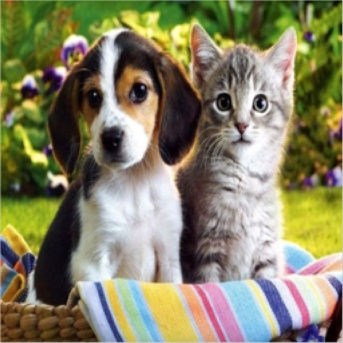
\includegraphics[width=0.14\linewidth,height=0.115\linewidth]{figs/examples/googlenet/oxford/dog-cat2} &
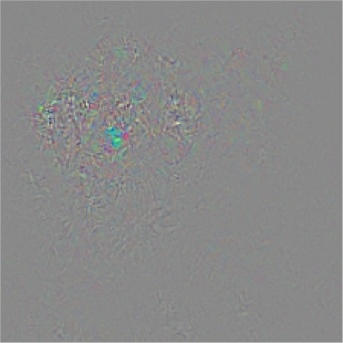
\includegraphics[width=0.14\linewidth,height=0.115\linewidth]{figs/examples/googlenet/oxford/dog-cat2_diff_163} &
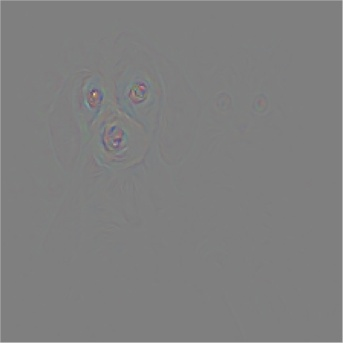
\includegraphics[width=0.14\linewidth,height=0.115\linewidth]{figs/examples/googlenet/deconv/dog-cat2_diff_163} &
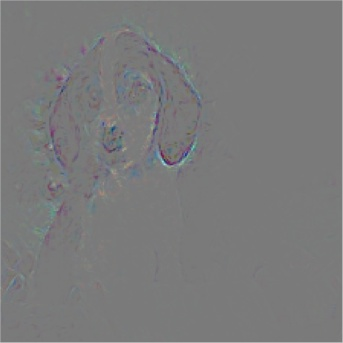
\includegraphics[width=0.14\linewidth,height=0.115\linewidth]{figs/examples/googlenet/soft/dog-cat2_diff_163} &
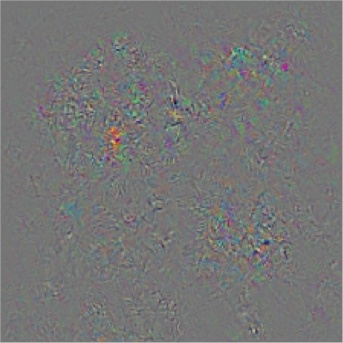
\includegraphics[width=0.14\linewidth,height=0.115\linewidth]{figs/examples/googlenet/oxford/dog-cat2_diff_286} &
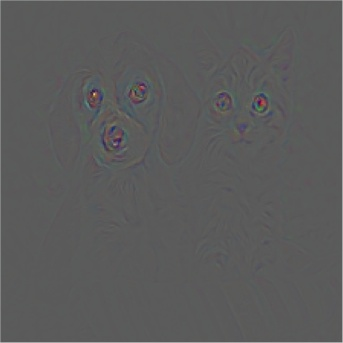
\includegraphics[width=0.14\linewidth,height=0.115\linewidth]{figs/examples/googlenet/deconv/dog-cat2_diff_286} &
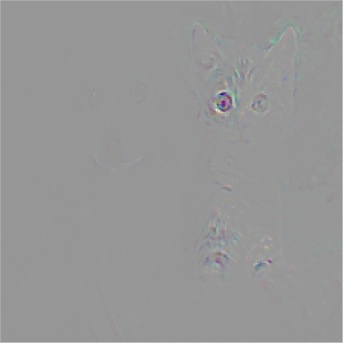
\includegraphics[width=0.14\linewidth,height=0.115\linewidth]{figs/examples/googlenet/soft/dog-cat2_diff_286} \\
\vspace{-2.5pt}
%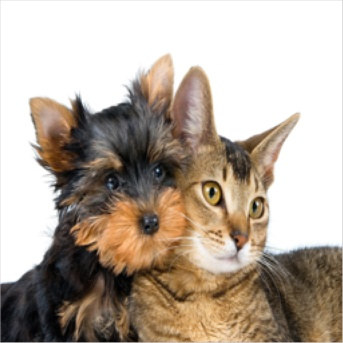
\includegraphics[width=0.14\linewidth,height=0.115\linewidth]{figs/examples/googlenet/oxford/dog-cat3} &
%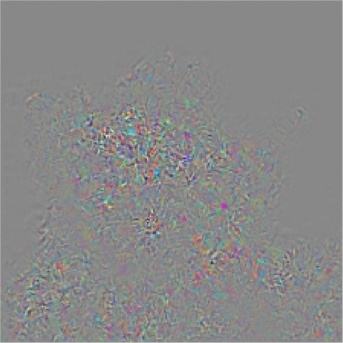
\includegraphics[width=0.14\linewidth,height=0.115\linewidth]{figs/examples/googlenet/oxford/dog-cat3_diff_188} &
%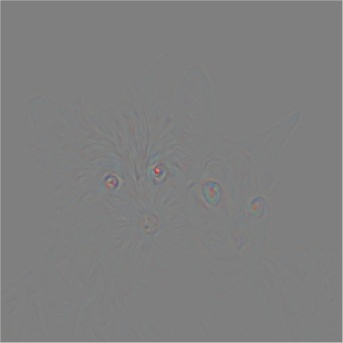
\includegraphics[width=0.14\linewidth,height=0.115\linewidth]{figs/examples/googlenet/deconv/dog-cat3_diff_188} &
%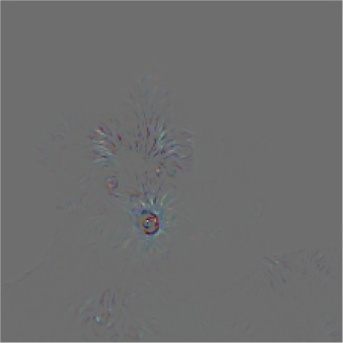
\includegraphics[width=0.14\linewidth,height=0.115\linewidth]{figs/examples/googlenet/soft/dog-cat3_diff_188} &
%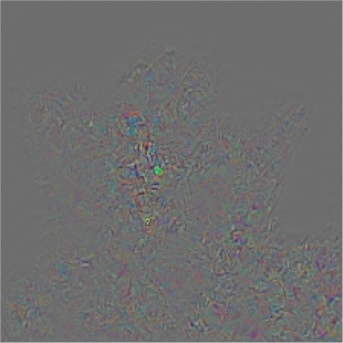
\includegraphics[width=0.14\linewidth,height=0.115\linewidth]{figs/examples/googlenet/oxford/dog-cat3_diff_286} &
%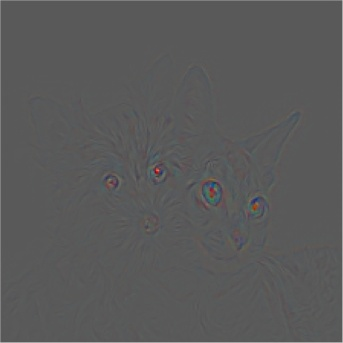
\includegraphics[width=0.14\linewidth,height=0.115\linewidth]{figs/examples/googlenet/deconv/dog-cat3_diff_286} &
%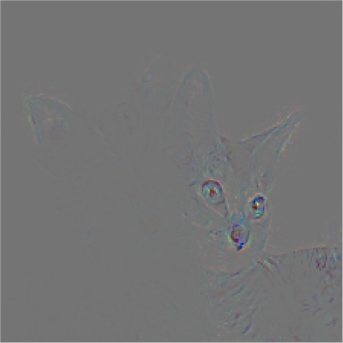
\includegraphics[width=0.14\linewidth,height=0.115\linewidth]{figs/examples/googlenet/soft/dog-cat3_diff_286} \\
%\vspace{-2.5pt}
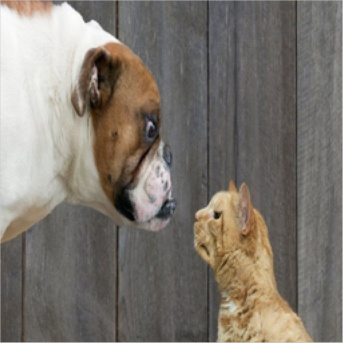
\includegraphics[width=0.14\linewidth,height=0.115\linewidth]{figs/examples/googlenet/oxford/dog-cat4} &
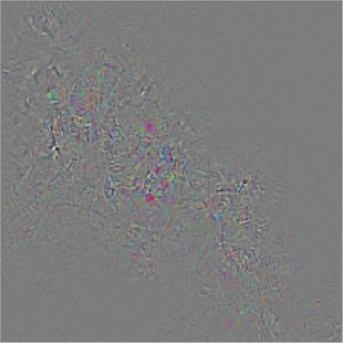
\includegraphics[width=0.14\linewidth,height=0.115\linewidth]{figs/examples/googlenet/oxford/dog-cat4_diff_243} &
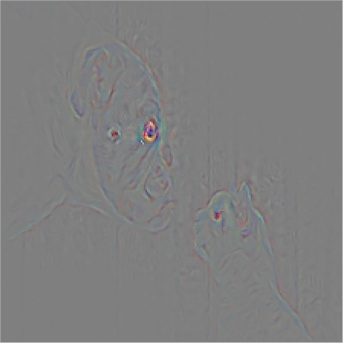
\includegraphics[width=0.14\linewidth,height=0.115\linewidth]{figs/examples/googlenet/deconv/dog-cat4_diff_243} &
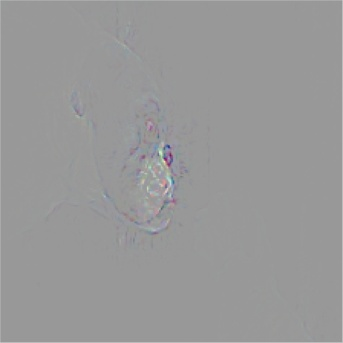
\includegraphics[width=0.14\linewidth,height=0.115\linewidth]{figs/examples/googlenet/soft/dog-cat4_diff_243} &
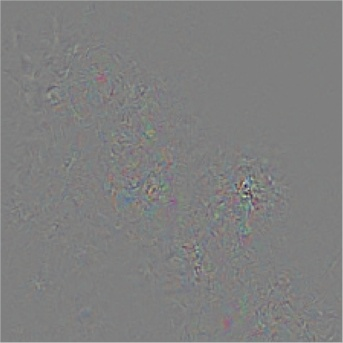
\includegraphics[width=0.14\linewidth,height=0.115\linewidth]{figs/examples/googlenet/oxford/dog-cat4_diff_286} &
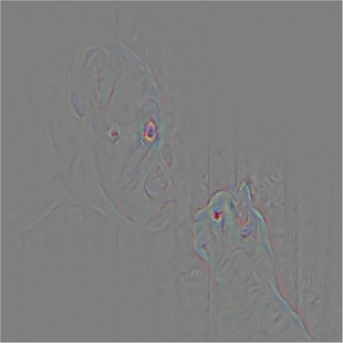
\includegraphics[width=0.14\linewidth,height=0.115\linewidth]{figs/examples/googlenet/deconv/dog-cat4_diff_286} &
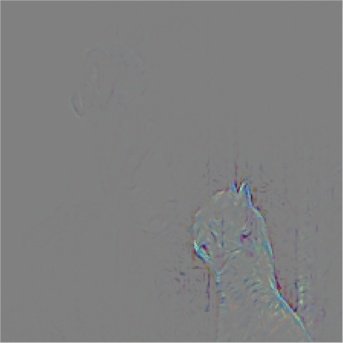
\includegraphics[width=0.14\linewidth,height=0.115\linewidth]{figs/examples/googlenet/soft/dog-cat4_diff_286} \\
& \multicolumn{3}{c}{\small -------------------- Object 1: car --------------------} & \multicolumn{3}{c}{\small -------------------- Object 2: bike --------------------} \\
\vspace{-2.5pt}
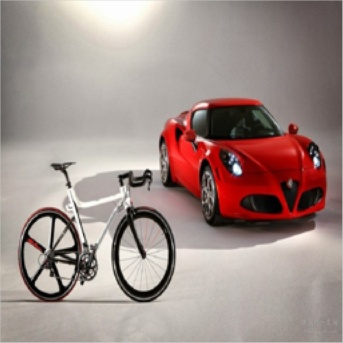
\includegraphics[width=0.14\linewidth,height=0.115\linewidth]{figs/examples/googlenet/oxford/bic-car1} &
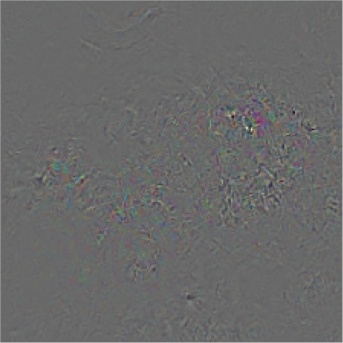
\includegraphics[width=0.14\linewidth,height=0.115\linewidth]{figs/examples/googlenet/oxford/bic-car1_diff_818} &
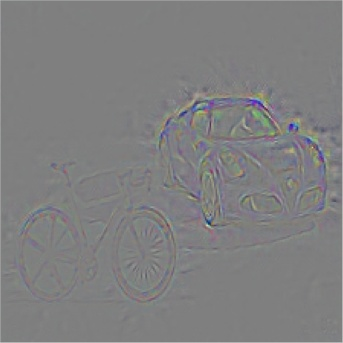
\includegraphics[width=0.14\linewidth,height=0.115\linewidth]{figs/examples/googlenet/deconv/bic-car1_diff_818} &
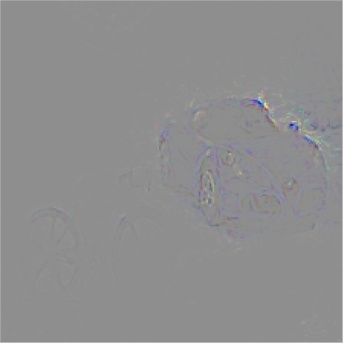
\includegraphics[width=0.14\linewidth,height=0.115\linewidth]{figs/examples/googlenet/soft/bic-car1_diff_818} &
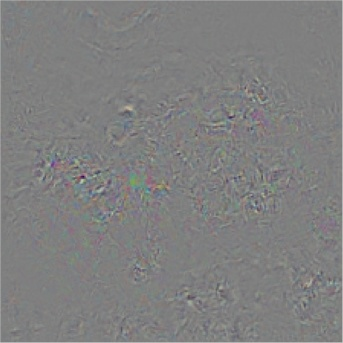
\includegraphics[width=0.14\linewidth,height=0.115\linewidth]{figs/examples/googlenet/oxford/bic-car1_diff_672} &
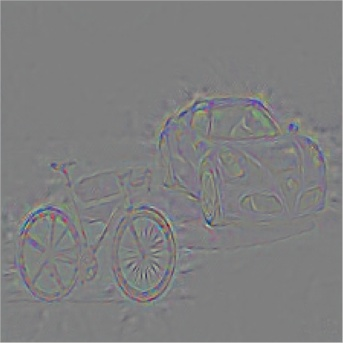
\includegraphics[width=0.14\linewidth,height=0.115\linewidth]{figs/examples/googlenet/deconv/bic-car1_diff_672} &
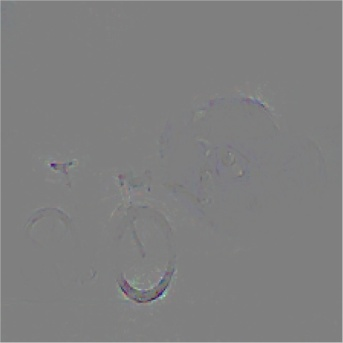
\includegraphics[width=0.14\linewidth,height=0.115\linewidth]{figs/examples/googlenet/soft/bic-car1_diff_672} \\
\vspace{-2.5pt}
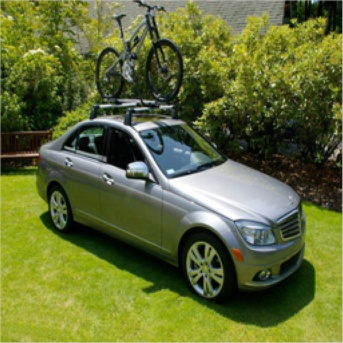
\includegraphics[width=0.14\linewidth,height=0.115\linewidth]{figs/examples/googlenet/oxford/bic-car2} &
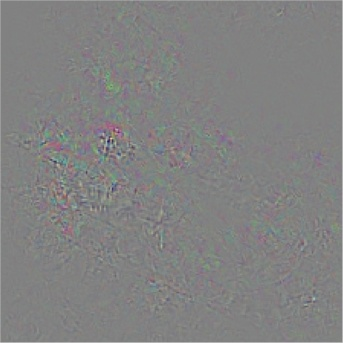
\includegraphics[width=0.14\linewidth,height=0.115\linewidth]{figs/examples/googlenet/oxford/bic-car2_diff_818} &
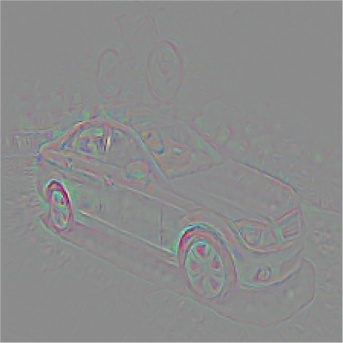
\includegraphics[width=0.14\linewidth,height=0.115\linewidth]{figs/examples/googlenet/deconv/bic-car2_diff_818} &
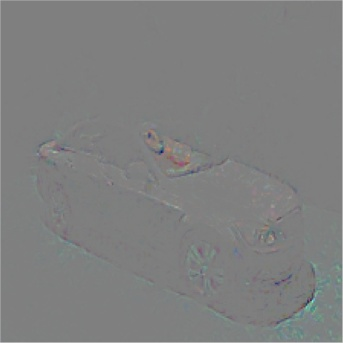
\includegraphics[width=0.14\linewidth,height=0.115\linewidth]{figs/examples/googlenet/soft/bic-car2_diff_818} &
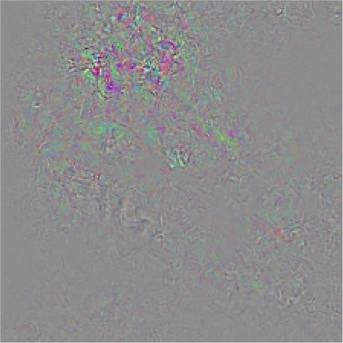
\includegraphics[width=0.14\linewidth,height=0.115\linewidth]{figs/examples/googlenet/oxford/bic-car2_diff_672} &
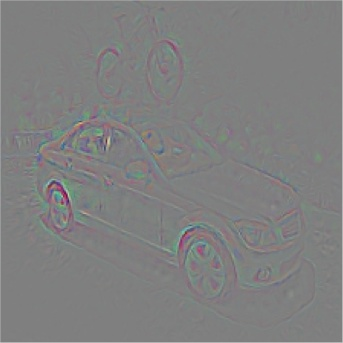
\includegraphics[width=0.14\linewidth,height=0.115\linewidth]{figs/examples/googlenet/deconv/bic-car2_diff_672} &
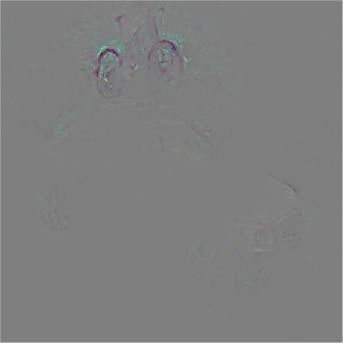
\includegraphics[width=0.14\linewidth,height=0.115\linewidth]{figs/examples/googlenet/soft/bic-car2_diff_672} \\
& \multicolumn{3}{c}{\small -------------------- Object 1: zebra --------------------} & \multicolumn{3}{c}{\small -------------------- Object 2: elephant --------------------} \\
\vspace{-2.5pt}
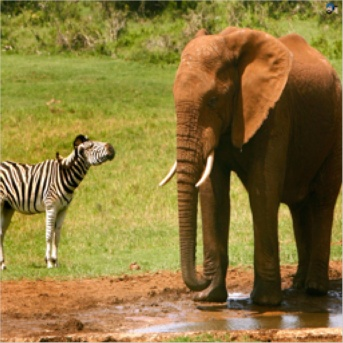
\includegraphics[width=0.14\linewidth,height=0.115\linewidth]{figs/examples/googlenet/oxford/zeb-ele1} &
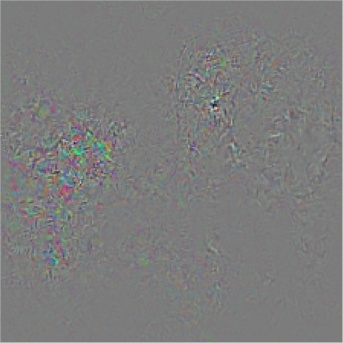
\includegraphics[width=0.14\linewidth,height=0.115\linewidth]{figs/examples/googlenet/oxford/zeb-ele1_diff_341} &
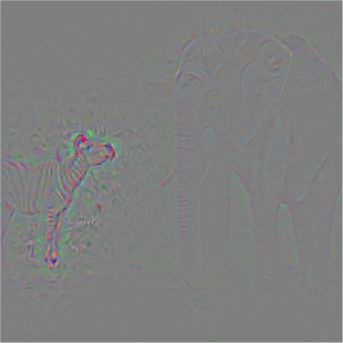
\includegraphics[width=0.14\linewidth,height=0.115\linewidth]{figs/examples/googlenet/deconv/zeb-ele1_diff_341} &
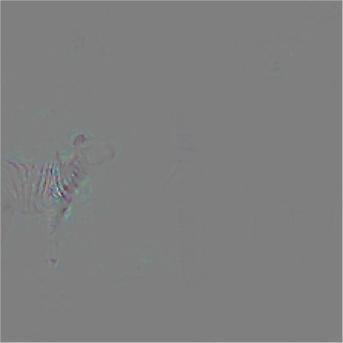
\includegraphics[width=0.14\linewidth,height=0.115\linewidth]{figs/examples/googlenet/soft/zeb-ele1_diff_341} &
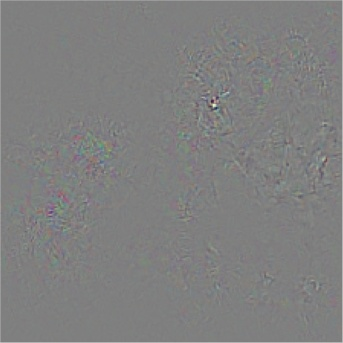
\includegraphics[width=0.14\linewidth,height=0.115\linewidth]{figs/examples/googlenet/oxford/zeb-ele1_diff_387} &
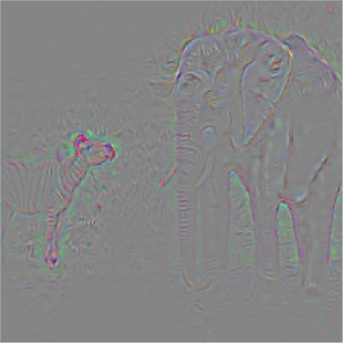
\includegraphics[width=0.14\linewidth,height=0.115\linewidth]{figs/examples/googlenet/deconv/zeb-ele1_diff_387} &
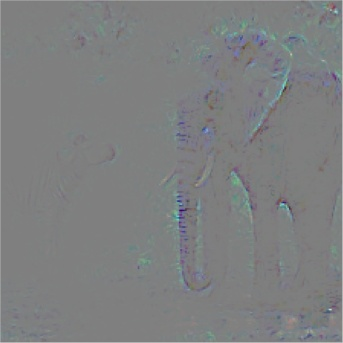
\includegraphics[width=0.14\linewidth,height=0.115\linewidth]{figs/examples/googlenet/soft/zeb-ele1_diff_387} \\
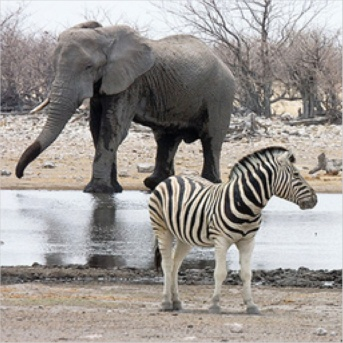
\includegraphics[width=0.14\linewidth,height=0.115\linewidth]{figs/examples/googlenet/oxford/zeb-ele2} &
\includegraphics[width=0.14\linewidth,height=0.115\linewidth]{figs/examples/googlenet/oxford/zeb-ele2_diff_341} &
\includegraphics[width=0.14\linewidth,height=0.115\linewidth]{figs/examples/googlenet/deconv/zeb-ele2_diff_341} &
\includegraphics[width=0.14\linewidth,height=0.115\linewidth]{figs/examples/googlenet/soft/zeb-ele2_diff_341} &
\includegraphics[width=0.14\linewidth,height=0.115\linewidth]{figs/examples/googlenet/oxford/zeb-ele2_diff_387} &
\includegraphics[width=0.14\linewidth,height=0.115\linewidth]{figs/examples/googlenet/deconv/zeb-ele2_diff_387} &
\includegraphics[width=0.14\linewidth,height=0.115\linewidth]{figs/examples/googlenet/soft/zeb-ele2_diff_387} \\
{\small (a) Image} &
{\small (b) Gradient} &
{\small (c) Deconv} &
{\small (d) Feedback} &
{\small (e) Gradient} &
{\small (f) Deconv} &
{\small (g) Feedback} \\
\end{tabular}
% \vspace{-10pt}
\caption{We demonstrate the effectiveness of feedback neural networks for class-specific feature extraction, by comparing the class model visualization results against original gradient~\cite{simonyan2013deep} and Deconv~\cite{zeiler2014visualizing} on selected images with multiple objects. All methods compute visualizations using a pre-trained GoogleNet trained on ImageNet 2012 classification dataset. Column (a) shows the input images (\emph{i.e.} dog v.s. cat, car v.s. bike, and zebra v.s. elephant). Column (b) and (e) show the original image gradients given the provided class labels. Column (c) and (f) show the Deconv results. Column (d) and (g) show the image gradients after feedback. Comparing against original gradient and Deconv, the feedback visualization captures more accurate salient area of the target object. For example, in the 4th row, both original template and Deconv see the dog and cat, even provided with the target label. In the last row, when zebra is specified, Deconv finds it hard to suppress the elephant area. Our feedback method suppress the irrelevant object much better. Better viewed in color and zoom in.}
\label{fig:examples}
% \vspace{-30pt}
\end{center}
\end{figure*}

The \emph{Feedback Network} could be used to improve various computer vision problems. In this paper, we demonstrate its potential, conduct qualitative experiments on class neuron visualizations, and quantitative experiments on weakly supervised object localization task. Furthermore, we show that the image recognition could also benefit from the \emph{Feedback} mechanism, by taking the strategy ``Looking and Thinking Twice'', which eliminate noisy or cluttered background and makes the network focused on salient regions.
We use three most popular pre-trained ConvNet models, AlexNet~\cite{Krizhevsky2012ImageNet}, VggNet~\cite{simonyan2013deep} and GoogleNet~\cite{Szegedy2014Going} for experiments. All three models are pre-trained with ImageNet 2012 classification training dataset~\cite{deng2009imagenet}, obtained from Caffe~\cite{jia2014caffe} model zoo\footnote{https://github.com/BVLC/caffe/wiki/Model-Zoo}.
% I think this sentence has no effect here. Remove it.
% AlexNet achieves $\sim$15\% top 5 classification error on ImageNet 2012 testing dataset, while VggNet and GoogleNet obtains $\sim$7.5\%. GoogleNet slightly outperforms VggNet, but the gap is small and can be ignored.

\subsection{Image Specific Class Model Visualization}
\label{subsec:visualization}
Given an image $I$, a class label $k$ and the hidden neuron activation states $\mathbf{z}$, we approximate the neural net class score $s_k$ with the first-order taylor expansion in the neighborhood of $I$:
\begin{equation}
  s_k(I, \mathbf{z}) \approx  \mathbf{T}_k(\mathbf{z})^T I + b
\end{equation}
where $\mathbf{T}_k(\mathbf{z})$ is the derivative of $s_k$ with respect to the image at the point of $I$ and $\mathbf{z}$. $\mathbf{T}_k(\mathbf{z})$ can be viewed as the linear template applied on image $I$ for measuring how likely the image belongs to class $k$, and could be visualized in the same spatial space since it is of the same size as input image $I$.
% We can visualize $\mathbf{T}$ since it's of the same size as the image $I$.
We use this technique to visualize our feedback model throughout the paper.

% What is this sentence saying??? I don't understand! Why only VggNet???
More specifically, for a Convolutional Network composed with a stack of piecewise linear layers (\emph{i.e.} Conv, ReLU and max-pooling) to compute the class scores, once the hidden states $\mathbf{z}$ are determined, the final score is a linear function of the image, which is equivalent to the inner product between the template and the image.

\textbf{Comparison of Visualization Methods:} We compare the image gradient (template $\mathbf{T}$) after the feedback process against the original one in feedforward pass, and Deconvolutional Neural Net~\cite{zeiler2014visualizing} on a set of complex images containing multiple objects from different classes, with all using the same pre-trained GoogleNet and being given ground truth class labels as a prior. Qualitative results are shown in Figure~\ref{fig:examples}. Without involving the feedback, where all hidden neurons' status are determined by the bottom-up computation only, the visualization is the same as original image gradient. However, compared with Deconv-like approaches, our feedback model is more efficient in capturing salient regions for each specific class while suppress those irrelevant object areas at the same time after feedback.

\textbf{Comparison of ConvNet Models:} We also qualitatively compare major convolutional network models, \emph{i.e.}, AlexNet, VggNet and GoogleNet, by visualizing their feedback templates in Figure~\ref{fig:model_compare}. All models are given ground truth  labels a prior. From visualizations, we find that VggNet and GoogleNet produce more accurate visual attention than AlexNet, suggesting that using smaller convolution filters and deeper architectures could further distinguish similar and nearby objects. Moreover, although both VggNet and GoogleNet produce very similar image classification accuracies, GoogleNet better captures the salient object areas than VggNet. We hypothesize that the two $4,096$ dimensional fully connected layers (\emph{i.e.}, fc6, fc7) in VggNet (which GoogleNet does not contain) could ruin the spatial distinctiveness of image features, as pointed out in~\cite{lin2013network}.

%%===========================================================
%% Revision in camera-ready version: remove gradient visualizations and preserve only the salience maps
%%===========================================================
\setlength{\tabcolsep}{0.5pt}
\begin{figure*}
\begin{center}
\begin{tabular}{ccccccc}
%\rotatebox{90}{\hspace{5mm}Gradient} &
%\vspace{-2.5pt}
%\includegraphics[width=0.14\linewidth,height=0.115\linewidth]{figs/examples/googlenet/soft/zeb-ele1} &
%\includegraphics[width=0.14\linewidth,height=0.115\linewidth]{figs/examples/alexnet/soft/zeb-ele1_diff_341} &
%\includegraphics[width=0.14\linewidth,height=0.115\linewidth]{figs/examples/vggnet/soft/zeb-ele1_diff_341} &
%\includegraphics[width=0.14\linewidth,height=0.115\linewidth]{figs/examples/googlenet/soft/zeb-ele1_diff_341} &
%\includegraphics[width=0.14\linewidth,height=0.115\linewidth]{figs/examples/alexnet/soft/zeb-ele1_diff_387} &
%\includegraphics[width=0.14\linewidth,height=0.115\linewidth]{figs/examples/vggnet/soft/zeb-ele1_diff_387} &
%\includegraphics[width=0.14\linewidth,height=0.115\linewidth]{figs/examples/googlenet/soft/zeb-ele1_diff_387} \\
%\rotatebox{90}{\hspace{5mm}Saliency} &
\vspace{-2.5pt}
\includegraphics[width=0.14\linewidth,height=0.115\linewidth]{figs/examples/googlenet/soft/zeb-ele1} &
\includegraphics[width=0.14\linewidth,height=0.115\linewidth]{figs/examples/alexnet/soft/zeb-ele1_sali_341} &
\includegraphics[width=0.14\linewidth,height=0.115\linewidth]{figs/examples/vggnet/soft/zeb-ele1_sali_341} &
\includegraphics[width=0.14\linewidth,height=0.115\linewidth]{figs/examples/googlenet/soft/zeb-ele1_sali_341} &
\includegraphics[width=0.14\linewidth,height=0.115\linewidth]{figs/examples/alexnet/soft/zeb-ele1_sali_387} &
\includegraphics[width=0.14\linewidth,height=0.115\linewidth]{figs/examples/vggnet/soft/zeb-ele1_sali_387} &
\includegraphics[width=0.14\linewidth,height=0.115\linewidth]{figs/examples/googlenet/soft/zeb-ele1_sali_387} \\
%\rotatebox{90}{\hspace{5mm}Gradient} &
%\vspace{-2.5pt}
%\includegraphics[width=0.14\linewidth,height=0.115\linewidth]{figs/examples/googlenet/soft/zeb-ele2} &
%\includegraphics[width=0.14\linewidth,height=0.115\linewidth]{figs/examples/alexnet/soft/zeb-ele2_diff_341} &
%\includegraphics[width=0.14\linewidth,height=0.115\linewidth]{figs/examples/vggnet/soft/zeb-ele2_diff_341} &
%\includegraphics[width=0.14\linewidth,height=0.115\linewidth]{figs/examples/googlenet/soft/zeb-ele2_diff_341} &
%\includegraphics[width=0.14\linewidth,height=0.115\linewidth]{figs/examples/alexnet/soft/zeb-ele2_diff_387} &
%\includegraphics[width=0.14\linewidth,height=0.115\linewidth]{figs/examples/vggnet/soft/zeb-ele2_diff_387} &
%\includegraphics[width=0.14\linewidth,height=0.115\linewidth]{figs/examples/googlenet/soft/zeb-ele2_diff_387} \\
%\rotatebox{90}{\hspace{5mm}Saliency} &
\includegraphics[width=0.14\linewidth,height=0.115\linewidth]{figs/examples/googlenet/soft/zeb-ele2} &
\includegraphics[width=0.14\linewidth,height=0.115\linewidth]{figs/examples/alexnet/soft/zeb-ele2_sali_341} &
\includegraphics[width=0.14\linewidth,height=0.115\linewidth]{figs/examples/vggnet/soft/zeb-ele2_sali_341} &
\includegraphics[width=0.14\linewidth,height=0.115\linewidth]{figs/examples/googlenet/soft/zeb-ele2_sali_341} &
\includegraphics[width=0.14\linewidth,height=0.115\linewidth]{figs/examples/alexnet/soft/zeb-ele2_sali_387} &
\includegraphics[width=0.14\linewidth,height=0.115\linewidth]{figs/examples/vggnet/soft/zeb-ele2_sali_387} &
\includegraphics[width=0.14\linewidth,height=0.115\linewidth]{figs/examples/googlenet/soft/zeb-ele2_sali_387} \\
%\rotatebox{90}{\hspace{5mm}Gradient} &
%\includegraphics[width=0.13\linewidth]{figs/examples/googlenet/soft/bic-car1} &
%\includegraphics[width=0.13\linewidth]{figs/examples/alexnet/soft/bic-car1_diff_818} &
%\includegraphics[width=0.13\linewidth]{figs/examples/vggnet/soft/bic-car1_diff_818} &
%\includegraphics[width=0.13\linewidth]{figs/examples/googlenet/soft/bic-car1_diff_818} &
%\includegraphics[width=0.13\linewidth]{figs/examples/alexnet/soft/bic-car1_diff_672} &
%\includegraphics[width=0.13\linewidth]{figs/examples/vggnet/soft/bic-car1_diff_672} &
%\includegraphics[width=0.13\linewidth]{figs/examples/googlenet/soft/bic-car1_diff_672} \\
%\rotatebox{90}{\hspace{5mm}Saliency} &
%\includegraphics[width=0.13\linewidth]{figs/examples/googlenet/soft/bic-car1} &
%\includegraphics[width=0.13\linewidth]{figs/examples/alexnet/soft/bic-car1_sali_818} &
%\includegraphics[width=0.13\linewidth]{figs/examples/vggnet/soft/bic-car1_sali_818} &
%\includegraphics[width=0.13\linewidth]{figs/examples/googlenet/soft/bic-car1_sali_818} &
%\includegraphics[width=0.13\linewidth]{figs/examples/alexnet/soft/bic-car1_sali_672} &
%\includegraphics[width=0.13\linewidth]{figs/examples/vggnet/soft/bic-car1_sali_672} &
%\includegraphics[width=0.13\linewidth]{figs/examples/googlenet/soft/bic-car1_sali_672} \\
%\rotatebox{90}{\hspace{5mm}Gradient} &
%\includegraphics[width=0.13\linewidth]{figs/examples/googlenet/soft/bic-car2} &
%\includegraphics[width=0.13\linewidth]{figs/examples/alexnet/soft/bic-car2_diff_818} &
%\includegraphics[width=0.13\linewidth]{figs/examples/vggnet/soft/bic-car2_diff_818} &
%\includegraphics[width=0.13\linewidth]{figs/examples/googlenet/soft/bic-car2_diff_818} &
%\includegraphics[width=0.13\linewidth]{figs/examples/alexnet/soft/bic-car2_diff_672} &
%\includegraphics[width=0.13\linewidth]{figs/examples/vggnet/soft/bic-car2_diff_672} &
%\includegraphics[width=0.13\linewidth]{figs/examples/googlenet/soft/bic-car2_diff_672} \\
%\rotatebox{90}{\hspace{5mm}Saliency} &
%\includegraphics[width=0.13\linewidth]{figs/examples/googlenet/soft/bic-car2} &
%\includegraphics[width=0.13\linewidth]{figs/examples/alexnet/soft/bic-car2_sali_818} &
%\includegraphics[width=0.13\linewidth]{figs/examples/vggnet/soft/bic-car2_sali_818} &
%\includegraphics[width=0.13\linewidth]{figs/examples/googlenet/soft/bic-car2_sali_818} &
%\includegraphics[width=0.13\linewidth]{figs/examples/alexnet/soft/bic-car2_sali_672} &
%\includegraphics[width=0.13\linewidth]{figs/examples/vggnet/soft/bic-car2_sali_672} &
%\includegraphics[width=0.13\linewidth]{figs/examples/googlenet/soft/bic-car2_sali_672} \\
{\small (a) Image} &
{\small (b) AlexNet} &
{\small (c) VggNet} &
{\small (d) GoogleNet} &
{\small (e) AlexNet} &
{\small (f) VggNet} &
{\small (g) GoogleNet} \\
\end{tabular}
% \vspace{-10pt}
\caption{We visualize the feedback ability of three most popular pre-trained ConvNets: AlexNet, VggNet and GoogleNet, by visualizing final image gradients and salience maps after feedback. We show the input images in column (a); results of these three models feedbacked by "zebra" are shown in column (b), (c), (d), and by "elephant" in column (e), (f), (g) respectively. We find that VggNet performs quite better than AlexNet, especially in capturing salient object details, suggesting the benefit of usage of small convolutional filters and deeper architecture. Although both VggNet and GogoleNet produce similar classification accuracy, GoogleNet provides the better class specific feature separations according to these results. We suspect the two 4096 fully connected layers in VggNet (which GoogleNet does not have) may harm the spatial distinctiveness of image features.}
\label{fig:model_compare}
% \vspace{-30pt}
\end{center}
\end{figure*}


\subsection{Weakly Supervised Object Localization}
\label{subsec:localization}

\begin{table}[htb]
\centering
\small
% Localization Errors Given Ground Truth Labels
\begin{tabular}{|c|c|}
\hline
Method & Localization Error (\%) \\ \hline
Oxford~\cite{simonyan2013deep} & 44.6 \\ \hline
%Deconv~\cite{zeiler2014visualizing} & 46.9 \\ \hline
Feedback & \textbf{38.8} \\ \hline
%Oxford-Supervised~\cite{Simonyan2014Very} & 34.3 \\ \hline
\end{tabular}
\caption{Comparison of our weakly supervised localization results on ImageNet 2014 localization validation set with the simplified testing protocol: the bounding box is predicted from a single central crop of images and the ground truth labels are provided.
We show that our feedback method significant outperforms the baseline method (error rate 44.6\%) that uses the original image gradient to localize in \cite{simonyan2013deep}, both on GoogLeNet architecture.
%We show that our feedback method significantly outperforms the baseline method (44.6\%) that uses the original image gradient to localize, and works even closer to a carefully trained supervised localization model (34.3\%).
}
\label{tab:localization_accuracy}
\end{table}

\begin{table}[htb]
\centering
\small
% Localization Errors of Different Feedback ConvNets
\begin{tabular}{c|c|c}
\hline
                                      & Weakly Supervised             & Supervised              \\ \hline
Model                                 & Localization Error (\%)       & Localization Error (\%) \\ \hline
AlexNet~\cite{Krizhevsky2012ImageNet} & 49.6                          & -                       \\ \hline
VggNet~\cite{Simonyan2014Very}        & 40.2                          & 34.3\cite{Simonyan2014Very} \\ \hline
GooglNet~\cite{Szegedy2014Going}      & \textbf{38.8}                 & - \\ \hline
\end{tabular}
\caption{Column 2 compares localization errors using feedback on different ConvNet models. VGG and GoogleNet significant outperform AlexNet suggesting they are learning better features. GoogleNet outperforms VGG even further, which matches the observations in Figure~\ref{fig:model_compare}. We also compare the weakly-supervised feedback mechanism with totally supervised localization model in \cite{Simonyan2014Very} on VGG, in the third column. It shows that we are competitive to a carefully trained localization model (34.3\%) using pixel-wise supervised training data.}
\label{tab:localization_model_compare}
\end{table}

To quantitatively demonstrate the effectiveness of the feedback model. we experiment on the ImageNet 2014 localization task. As pointed in~\cite{simonyan2013deep}, the magnitude of the elements in the model template $\mathbf{T}_k$ defines the class specific salience map on image $I$. Pixels with larger magnitudes indicate that they are more important to the class. We adopt the same saliency extraction strategy as~\cite{simonyan2013deep} that a single class saliency value $M_k$ for class $k$ at pixel $(i,j)$ is computed across all color channels: $M_k(i,j) = \max_{c \in rgb} | T_k(i,j,c) |$.

We show that the proposed Feedback CNN has the potential to unify recognition and detection into a single network architecture in this experiment, instead of using separate ones to perform different tasks respectively. Although the three ConvNets are pre-trained for image classification, we could use the feedbacked salience map for weakly supervised object localization. Given an image and the corresponding class salience map, we compute the object segmentation mask by simply thresholding so that the foreground area covers $95\%$ energy out of the whole salience map, and calculate a tightest bounding box as the localization result. Different from~\cite{simonyan2013deep}, which uses GraphCut~\cite{yuri2001interactive}, this requires saliency maps of higher quality, but only takes less computation.

We test our localization results on ImageNet 2014 localization validation set, which contains $\sim50,000$ images with each image associated with labels and corresponding bounding boxes. A prediction is considered as correct if and only if its overlap with the ground truth bounding box is over 50\%. Image are resized  to 224x224 to meet the model requirement on resolutions, and ground-truth class labels are provided to predict localizations. Neither further preprocessing nor multi-scale strategy are involved.

\textbf{Comparison of Localization Methods:} Table~\ref{tab:localization_accuracy} shows the comparison of our weakly supervised localization accuracy against the baseline method~\cite{simonyan2013deep}. For fair comparison, we reimplemented the method in~\cite{simonyan2013deep} following the details in the original paper strictly, and name as ``Oxford.'' For our method, we use GoogLeNet and apply the same segmentation strategy in our model. Our method obtains 38.8\% localization error, and significantly outperforms Oxford (44.6\%), suggesting that in terms of capturing attention and localizing salient objects, our feedback net is better. Note that our weakly supervised localization error is even closer to a carefully trained supervised localization model (34.3\%).

\textbf{Comparsion of ConvNet Models:} We also analyze weakly supervised localization accuracies of above mentioned three ConvNets in Table~\ref{tab:localization_model_compare}, provided with the same testing protocol. Even provided with ground truth class, VggNet and GoogleNet significantly outperforms AlexNet.
This suggests that better feature representations are sharable between the two highly correlated visual tasks: recognition and localization. GoogLeNet outperforms VggNet even further, which matches the observations in Figure~\ref{fig:model_compare}.

\subsection{Image Re-Classification with Attention}
\label{subsec:re-classification}

\begin{table}
\centering
\small
\begin{tabular}{|c|c|c|}
\hline
Method & Top 1 (\%) & Top 5 (\%) \\ \hline
GoogleNet~\cite{Szegedy2014Going} & 32.28 & 11.75 \\ \hline
GoogleNet Feedback & \textbf{30.49} & \textbf{10.46} \\ \hline
\end{tabular}
\caption{Classification errors on ImageNet 2014 validation set with the simplified testing protocol: the first row is the performance of  GoogleNet given a single central crop of images, the second row shows classification results of the same GoogleNet given the attention cropped images, using the feedback mechanism in~\ref{subsec:re-classification}.}
\label{tab:reclassification_error}
\end{table}

Given the weakly supervised attention box, the image labels are {\em re-classified} using zoomed-in image patches cropped around the bounding box. We call such method {\em ``Look and Think Twice''}, which mimics the human visual recognition process that human may focus to recognize object in a complicated image after a first time glimpse. We apply this strategy to the image classification. By looking at the full image first in a coarse scale, our model obtains initial guesses of a set of most possible object classes, we then identify the salient object regions from the predicted top-ranked labels using the feedback neural nets, and re-classify those ROIs.

Here are the \textbf{Implementation Details}:
\begin{center}
  \fbox{
    \parbox{0.95\linewidth}{
      \noindent
      \begin{itemize}\itemsep2pt
        \item Resize image to size 224*224*3, run CNN model and predict top 5 class labels.
        \item \emph{Foreach} of the top 5 class labels, compute object localization box with feedback model.
        \item Crop image patch for each of 5 bounding boxes from original image and resize to $224*224*3$. Predict top 5 labels again.
        \item Given the total 25 labels and the corresponding confidences, rank them and pick the top 5 as final solution.
      \end{itemize}
    }
  }
\end{center}

\textbf{Classification Accuracy:} We test our classification results on ImageNet 2014 classification validation set, which contains $\sim50,000$ images with each image associated with one label. Table~\ref{tab:reclassification_error} shows the classification results using a pre-trained GoogleNet on the original full image and on the image patch based on feedback crop~\footnote{Model from Caffe Model Zoo}. After the re-classification, the top 5 classification errors drops by $1.29\%$, and, moreover, top 1 error improves even more $1.79\%$. These results suggest that correct estimations of bounding boxes by a glance can provide more accurate classifications.

\textbf{Ablative Study:} To further understand how ``Look and Think Twice'' improves the classification task, we divide the ImageNet 2014 localization validation set based on the proportion of the object size in the image. The ablative study is shown in Figure~\ref{fig:reclassification_delta}, and we find that classification errors drop using feedback crop for images with smaller objects, for example, for objects of less than $20\%$ area of images, the top-1 classification errors drop significantly with almost 5\%.
This phenomenon means traditional ConvNet is powerless in hanlding small objects because of cluttered backgrounds, while our algorithm could focus the network's attention onto those areas.

\setlength{\tabcolsep}{2pt}
\begin{figure}[htb]
\begin{center}
%\includegraphics[width=0.95\columnwidth]{figs/re-classification/re-classification}
\includegraphics[width=\columnwidth]{figs/re-classification/delta.pdf}
% \vspace{-10pt}
\caption{We divide the ImageNet 2014 localization validation set based on the proportion of the object size in the image. Classifications using feedback crop for images increase with smaller objects. E.g., for those images with object area smaller than 20\%, the top-1 classification accuracy increases significantly by almost 5\%.}
\label{fig:reclassification_delta}
%\vspace{-10pt}
\end{center}
\end{figure}

\setlength{\tabcolsep}{0.5pt}
\begin{figure}[htb]
\begin{center}
\begin{tabular}{ccc}
%\vspace{-2.5pt}
\includegraphics[width=0.31\linewidth,height=0.31\linewidth]{figs/re-classification/ILSVRC2012_val_00000115} &
\includegraphics[width=0.31\linewidth,height=0.31\linewidth]{figs/re-classification/boundingbox/ILSVRC2012_val_00000115} &
\includegraphics[width=0.31\linewidth,height=0.31\linewidth]{figs/re-classification/crop_image/ILSVRC2012_val_00000115} \\
%{\small 172, 264, 254, 265, 173} &
%{\small {\color{red} 174}, 216, 254, 181, 172} \\
\includegraphics[width=0.31\linewidth,height=0.31\linewidth]{figs/re-classification/ILSVRC2012_val_00000608} &
\includegraphics[width=0.31\linewidth,height=0.31\linewidth]{figs/re-classification/boundingbox/ILSVRC2012_val_00000608} &
\includegraphics[width=0.31\linewidth,height=0.31\linewidth]{figs/re-classification/crop_image/ILSVRC2012_val_00000608} \\
%{\small 837, 838, 448, 802, 634} &
%{\small 972, {\color{red} 644}, 634, 837, 573} \\
{\small (a) Original Image} &
{\small (b) Attention Boxes} &
{\small (c) Cropped Image} \\
\end{tabular}
% \vspace{-10pt}
\caption{We show two examples in the ImageNet localization validation set, demonstrating how the re-classification works. column (a) shows the original images which ConvNets predict incorrect labels ({\em "Italian greyhound"} and {\em "sunglass"}), column (b) shows the 5 calculated bounding box areas using the top-5 saliency maps, column (c) shows the cropped images obtained from the red box which ConvNets predict the correct labels ({\em "Ibizan hound"} and {\em "mask"}) with high confidences.}

\label{fig:reclassification_examples}
% \vspace{-30pt}
\end{center}
\end{figure}


